\chapter{成为小魔仙}

\begin{quote}
    羔羊揭开第七印的时候,天上寂静约有二刻……——《圣经·启示录》8:1
\end{quote}

在继续探索\LaTeX 这个庞大且出色的系统前,有必要停下脚步来了解一些重要的概念。实际上,为了成为能在组成这个系统的大量文件中大展身手的“赫尔克里·波洛”\yz{
    Hercule Poirot,阿加莎·克里斯蒂所著系列侦探小说中的主角。
},掌握这些概念是基本的要求。在本章,我们介绍有关计数器、长度、空白和字盒的内容。如果你在使用\LaTeX 时,除了顺从地使用它提供给你的格式外,还想要其他版式,这4个概念会很有用。

\begin{exclamation}
    本章涉及的概念有些微妙的细节,比较难以把握\jz{
        作者本人也不能保证掌握了全部内容……
    }。我们建议你实际上手体验一下,因为这里介绍的工具一方面可以为你生成最令人满意的结果,另一方面也能让你掉最多的头发,基本上跟直接在你头上薅差不多。
\end{exclamation}
\section{计数器}

文档中所有带有编号的对象都由\emph{计数器}生成。计数器可以递增、递减,也可以重设为0,等等。我们也可以根据自己的需要来创建计数器。

\subsection{可用的计数器}

计数器主要与标题、页码、浮动环境(环境\dm{figure}和\dm{table})、方程(环境\dm{equation})、页面底部的注释、编号列表(环境\dm{enumerate})息息相关。

表\ref{tab:4.1}列出了\LaTeX 中基础的计数器的名称。可以注意到,它们基本上都由相关对象的名称组成。计数器\dm{enumi}~\dm{enumiv}分别与环境\dm{enumerate}中的第1层~第4层相关。\dm{mpfootnote}是环境\dm{minipage}中脚注的计数器,会在4.4.3小节提到。

\begin{table}
  \centering
  \ttfamily
  \begin{tabular}{|l|l|l|l|}
    \hline
    part       & paragraph    & figure     & enumi\\
    chapter    & subparagraph & table      & enumii\\
    section    & page         & footnote   & enumiii\\
    subsection & equation     & mpfootnote & enumiv\\
    subsubsection &&&\\
    \hline
  \end{tabular}
  \caption{\LaTeX 的计数器}
  \label{tab:4.1}
\end{table}

\subsection{操作}

在接下来的段落中,我们介绍几个操作计数器的基本工具。注意,计数器是\emph{全局}变量,因此以下描述的三个指令也会在全局范围内生效。同时,也需要注意,其中的变量都是\emph{整数}。

\subsubsection{创建计数器}

可以通过以下指令\emph{创建}计数器:

\begin{dmd}
\backslash newcounter\{\codereplace{计数}\}[\codereplace{父计数}]
\end{dmd}

该指令可以创建一个新的计数器,名为\codereplace{计数}。参数\codereplace{父计数}是非强制的,如果配置,则每次\codereplace{父计数}递增时,\codereplace{计数}都会归零。

\subsubsection{指定计数}

可以通过以下方法为计数器指定一个值:

\begin{dmd}
\backslash setcounter\{\codereplace{计数}\}\{\codereplace{值}\}
\end{dmd}

其中,\codereplace{计数}代表我们想要指定值的计数器,\codereplace{值}即具体指定的值。

\subsubsection{增值}

可以通过以下指令使计数器的值增加或减少:

\begin{dmd}
  \backslash addtocounter\{\codereplace{计数}\}\{\codereplace{值}\}
\end{dmd}

其中,若\codereplace{值}为正数(对应地,负数),则可以使计数器的值增加(对应地,减少)。为了展现该指令的效果,我们在本书的文档中添加以下一行指令:

\begin{dmd}
\verb|\addtocounter{footnote}{357}|
\end{dmd}

\addtocounter{footnote}{357}
可以看到页面下方脚注的编号变化\jz{
  虽然这个值变了这么多属实有些荒谬……
}了。为了接下来的脚注恢复正确的序号,我们在源码中插入以下指令:

\begin{dmd}
  \verb|\addtocounter{footnote}{-357}|
\end{dmd}

\addtocounter{footnote}{-357}
可以看到,现在的脚注序号恢复正常\jz{
  天灵灵,地灵灵!
}了。

\subsection{显示}

使用如下指令可以将计数显示出来:

\begin{dmd}
\backslash the\codereplace{计数器名}
\end{dmd}

实际上,所有可以显示计数器的指令或环境都调用了类似的指令。这样一来,我们有如下指令:

\begin{itemize}
  \item \verb|\thepage|,在此处可以生成“\thepage ”,会在每次换页时调用;
  \item \verb|\thefootnote|,在此处可以生成“\thefootnote ”,会被\verb|\footnote|调用;
  \item \verb|\thesubsection|,在此处可以生成“\thesubsection ”,会被指令\verb|\subsection|调用;
  \item ……
\end{itemize}

“\verb|\the|”家族的指令通常借助以下格式指令定义:

\begin{itemize}
  \item \verb|\arabic{|\codereplace{计数器}\verb|}|;
  \item \verb|\roman{|\codereplace{计数器}\verb|}|和\verb|\Roman{|\codereplace{计数器}\verb|}|;
  \item \verb|\alph{|\codereplace{计数器}\verb|}|和\verb|\Alph{|\codereplace{计数器}\verb|}|。
\end{itemize}

以下是几个示例:

\begin{itemize}
  \item \verb|\arabic{page}|在此处可以生成“\arabic{page}”;
  \item \verb|\alph{footnote}|在此处可以生成“\alph{footnote}”,\verb|\Alph{section}|在此处可以生成“\Alph{section}”;
  \item \verb|\Roman{subsection}|在此处可以生成“\Roman{subsection}”,\verb|\roman{page}|在此处可以生成“\roman{page}”;
  \item ……
\end{itemize}

为了自定义文档,重定义“\verb|\the|”家族的指令的做法很常见。例如,在本书的文档中,指令\verb|\thefigure|以如下形式重定义:

\begin{dmd}
\verb|\arabic{chapter}.\arabic{figure}|
\end{dmd}

这样一来,本书的图题会依次以如下形式编号:

\begin{enumerate}
  \item 阿拉伯数字形式的章号;
  \item 圆点;
  \item 阿拉伯数字形式的图号。
\end{enumerate}

可以以如下的形式重新定义图题编号的显示形式。例如,以如下的形式定义:

\begin{dmd}
\verb|(\Roman{chapter}):\arabic{section}.\arabic{figure}|
\end{dmd}

这样可以在图题中以另一种形式——也是一种相对不整洁的形式——来为图编号。这里,我们重定义了指令\verb|\thefigure|,来生成新的编号方式:先在括号中以罗马数字形式显示章号,再以圆点分隔以阿拉伯数字形式显示的节号和图号。“\textsc{Fig.}”等字样、图号后的连接号等则需要在指令\verb|\caption|的层级去定义。

\begin{figure}[ht]
  \centering
  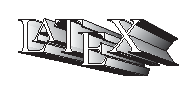
\includegraphics{img/latex.eps}\\
  \textsc{Figure} (IV):1.1: 特殊编号的图题
\end{figure}

\section{长度}

如果说计数器需要依托文档中对象的\emph{序号}而存在,那么长度就定义了实体\emph{占的空间}。长度是\LaTeX 中的一种参数,旨在以某种方式来表述对象的尺寸。

\subsection{单位}

所有的尺寸都需要带有单位。\emph{刚性}\jz{
  我们稍后会看到\emph{弹性}的尺寸。
}的尺寸具有如下形式:

\begin{dmd}
  \codereplace{数字}\codereplace{单位}
\end{dmd}

其中,\codereplace{数字}可以是正值或负值,在需要时也可以带小数;\codereplace{单位}需要是\LaTeX 可以识别的单位。可以使用包括但不仅限于如下列出的单位:

\begin{description}
  \item[cm] \emph{厘米};
  \item[mm] \emph{毫米};
  \item[in] \emph{英寸}(约\dm{2.54cm})\yz{
    目前,1英寸严格定义为2.54 cm,原文中的“约”不严谨。
  };
  \item[pt] \emph{点},通常在排版领域使用,合$\frac{1}{72.27}$英寸;
  \item[em] 当前字体下字母“M”的宽度;
  \item[ex] 当前字体下字母“x”的高度。
\end{description}

注意,单位\dm{em}(对应地,\dm{ex})一般会在水平(对应地,竖直)方向上衡量尺寸时使用,且使我们得以根据当前字体字号来决定尺寸。

\begin{table}[ht]
  \begin{tabular}{lcl}%todo现在是用字母凑的,看看能不能改成真的线段
    \dm{1cm} & : & \textsf{I}\!\rule{1cm}{1pt}\!\textsf{I} \\
    \dm{1in} & : & \textsf{I}\!\rule{1in}{1pt}\!\textsf{I} \\
    \dm{3mm} & : & \textsf{I}\!\rule{3mm}{1pt}\!\textsf{I} \\
    \dm{2em} & : & \textsf{I}\!\rule{2em}{1pt}\!\textsf{I} \\
    \dm{10pt} & : & \textsf{I}\!\rule{10pt}{1pt}\!\textsf{I} \\
  \end{tabular}
\end{table}


\subsection{\LaTeX 中的几个长度}

在\LaTeX 和各个扩展中都存在一些预定义的长度。这些长度一般决定了文档中某个部分的尺寸,例如:

\begin{itemize}
  \item \verb|\parindent|为段首缩进,默认为\dm{15pt};
  \item \verb|\textwidth|和\verb|\textheight|分别定义文本的宽度和高度;
  \item \verb|\baselineskip|定义了相邻两行间的基线距离(本书中为\dm{10pt}\yz{
    本项及下一项的具体尺寸都指原书。
  });
  \item \verb|\parskip|为段间距,初始化为\dm{0pt plus 1pt}\jz{
    关于\texttt{p}\texttt{lus}的含义,参见弹性尺寸部分。%连写plus一词会触发奇怪的编译不过bug
  };
  \item ……
\end{itemize}

需要理解,可以使用这些“内置”长度的函数来表示另一个长度,例如:

\begin{dmd}
\verb|0.5\textwidth|
\end{dmd}

这表示页面文本宽度的一半。再如:

\begin{dmd}
\verb|3\parindent|
\end{dmd}

这表示段间距的三倍。注意,对于长度\verb|-1\baselineskip|,可以直接将其写成\verb|-\baselineskip|。

\subsection{操作长度}

就像计数器,长度也可以使用一些指令来操作。

\subsubsection{创建长度}

以下指令可以创建一个长度:

\begin{dmd}
\backslash newlength\{\codereplace{尺寸}\}
\end{dmd}

其中\codereplace{尺寸}是该长度的名称。长度会被初始化为\dm{0pt}(参见示例4.1)。

\begin{exclamation}
注意,不论指令\verb|\newlength|出现在哪里,它的定义都是\textbf{全局的}。此外,一个长度被定义两次会引发报错。相反,对长度的修改是局部的,只会在它出现的组(\verb|{...}|)内生效。
\end{exclamation}

\subsubsection{指定长度}

可以使用以下指令来指定长度的值:

\begin{dmd}
\backslash setlength\{\codereplace{尺寸}\}\{\codereplace{值}\}
\end{dmd}

该指令可以将\codereplace{值}赋给\codereplace{尺寸}。

\subsubsection{增量}

可以使用以下方式来增加长度:

\begin{dmd}
\backslash alltolength\{\codereplace{尺寸}\}\{\codereplace{值}\}
\end{dmd}

该指令可以使\codereplace{尺寸}的值增加\codereplace{值}。

\addtolength{\parindent}{30pt} 在你读得正爽的时候,我们使用如下指令,冒昧地将长度\verb|\parindent|增加了30 pt:

\begin{dmd}
\verb+\addtolength{\parindent}{30pt}+ 在你读得正爽的时候,我们……
\end{dmd}

\addtolength{\parindent}{-30pt}
这样可以向你展示为长度增量的效果。在这之后,我们又写下了如下指令:

\begin{dmd}
\verb|\addtolength{\parindent}{-30pt}|
\end{dmd}

这样,接下来的缩进就又回到之前的样子了。

\subsubsection{获取对象尺寸}

\celan{\S 2.10}之前有模糊地提到过,在\TeX 层面上,组成文档的不同对象会被打包成\emph{字盒}。排列这些字盒时,实际上是将它们各自的\emph{参考点}码放整齐。这些码放整齐的点组成了一条虚拟的线,也就是该行文字的基线。所有的字盒都可以从以下三个维度衡量。

\begin{itemize}
  \item \emph{宽度}。
  \item \emph{高度}:从基线到字盒顶部的距离。
  \item \emph{深度}:从基线到字盒底部的距离。
\end{itemize}

例如,单词“Ingénierie”中,字盒的组合方式如下:

\newsavebox{\boitecar}
\newlength{\interletter}
\newlength{\letterwidth}
\newcommand{\refpoint}{\raisebox{-0.5\height}{\small$\circ$}}

\newcommand{\letterbox}[1]{%
   \setlength{\fboxsep}{0pt}%            
   \setlength{\fboxrule}{0.2pt}%            
   \sbox{\boitecar}{\framebox{\Huge#1}}%  
   \settowidth{\letterwidth}{\usebox{\boitecar}}%
   \settowidth{\interletter}{\Huge#1}%
   \makebox[0pt]{\refpoint}%
   \usebox{\boitecar}%
   \kern-\fboxrule%
}

\begin{center}
  \letterbox{\letterbox{I}%
  \letterbox{n}%
  \letterbox{g}%
  \letterbox{é}%
  \letterbox{n}%
  \letterbox{i}%
  \letterbox{e}%
  \letterbox{r}%
  \letterbox{i}%
  \letterbox{e}}
\end{center}

其中,符号“\refpoint”代表参考点。可以看到,除了带有字母“g”得字盒外,其他字盒的深度均为0。

但现在,我们还是先不接着说关于字盒的内容了!

借助以下指令,可以从对象(字母、单词、字盒等)中提取尺寸特征:

\begin{dmd}
\backslash settowidth\{\codereplace{尺寸}\}\{\codereplace{对象}\}\\
\backslash settoheight\{\codereplace{尺寸}\}\{\codereplace{对象}\}\\
\backslash settodepth\{\codereplace{尺寸}\}\{\codereplace{对象}\}
\end{dmd}

这三条指令分别将对象\codereplace{对象}的宽度、高度、深度指派给\codereplace{尺寸}。例如:

\begin{codelist}[4.1]{
\newlength{\malongueur}
\settowidth{\malongueur}{鸡零狗碎}
\begin{itemize}
\item 鸡零狗碎
\item \hspace{\malongueur}一地毛
\end{itemize}
}\begin{verbatim}
\newlength{\malongueur}
\settowidth{\malongueur}{鸡零狗碎}
\begin{itemize}
\item 鸡零狗碎
\item \hspace{\malongueur}一地毛
\end{itemize}
\end{verbatim}
\end{codelist}

长度\verb|\malongueur|代表了文字“鸡零狗碎”的宽度,被用作空格(参见关于\celan{\S 4.3}空格的段落)。

\subsection{弹性长度}

到目前为止,我们介绍的尺寸都属于\emph{刚性}尺寸\jz{
  除了\texttt{\backslash parskip}。
}。然而,还有一种\emph{弹性(élastiques或ressort)}长度。在\TeX 的层面,大量的尺寸都是以如下形式定义的:

\begin{dmd}
\codereplace{值} plus \codereplace{增值} plus \codereplace{减值}
\end{dmd}

这种语法可以定义一个尺寸\codereplace{值},但根据所处环境,它可以膨胀或缩小。也就是说,如果我们将创建的尺寸称为\codereplace{尺寸},则有

$$
\mbox{\codereplace{值}}-\mbox{\codereplace{减值}}\leqslant \mbox{\codereplace{尺寸}} \leqslant \mbox{\codereplace{值}}+\mbox{\codereplace{增值}}
$$

例如,长度\verb|\parskip|用于分隔相邻的段落,它被定为:

\begin{dmd}
0pt plus 1pt
\end{dmd}

这意味着,如果页面比较稀疏,\LaTeX 就会在段落之间增加1 pt垂直方向的空白。若要细微地调整水平或竖直方向上的距离,就很适合使用这种尺寸。此外,\LaTeX 的用户会有个奇特的机会,来处理另一类同样有趣的弹性长度。这类长度由以下两个特点:

\begin{itemize}
  \item 长度为\textbf{零};
  \item 可以在特定力的作用下\textbf{无限}伸长。
\end{itemize}

只要指明弹性的强弱,\LaTeXe 的指令就可以生成相应的弹性长度:

\begin{dmd}
\backslash stretch\{\codereplace{数字}\}
\end{dmd}

其中\codereplace{数字}代表弹力。这个数字可以带有符号,也可以是小数。以下是一个示例:

\begin{codelist}[4.2]{
  〇\hspace{\stretch{1}}%
三分点\hspace{\stretch{2}}一
}\begin{verbatim}
〇\hspace{\stretch{1}}%
三分点\hspace{\stretch{2}}一
\end{verbatim}
\end{codelist}

这段\LaTeX 代码在“〇”和“三分点”、“三分点”和“一”之间依据弹性长度生成了空间\jz{
  指令\texttt{\backslash hspace}生成了水平方向的空间,空间的长度取决于传入的参数。
},其中第二个空间的“僵硬”程度是第一个空间的两倍,对应地,空白占据了两倍的空间。此外需要注意,这种弹力是\emph{相对}但\emph{无限}的,因此,“〇”和“一”被“推”向了页面边缘。此外补充一点:\verb|\fill|是\verb|\stretch{1}|的简便写法。

\subsection{显示长度}

有时,显示长度的值十分有用。为了达成这个目的,可以借助指令\verb|\showthe|。该指令可以打断编译过程,并显示作为参数传入的长度的值,即:

\begin{dmd}
\verb|\showthe\linewidth|
\end{dmd}

该指令可以显示长度\verb|\linewidth|的值,同时打断\celan{\S 1.6}编译。我们可以在终端看到类似这样的信息:

\begin{dmd}
\begin{tabbing}
Document Class: book 2001/04/\= 21 v1.4 Standard LaTeX document\kill
\verb|[ ... ]| \> $\leftarrow$ \textsf{开头的一些套话}\\
Document Class: book 2001/04/21 v1.4 Standard LaTeX document\\
(/usr/share/texmf/tex/latex/base/bk12.clo)) (./test.aux)\\
> 17.62482pt. \> $\leftarrow$ \textsf{长度的值}\\
\verb|l.10 \showthe\parindent| \> $\leftarrow$ \textsf{要显示的长度}\\
~\\
?
\end{tabbing}
\end{dmd}

若编译是使用指令终端启动的,按\verb|<回车>|键就可以回到编译过程。

\begin{ii}
正如1.6节所说%TODO
,你使用的开发环境很可能不会显示来自\LaTeX 的消息。这种情况下,找到这些消息的任务就交给你了……
\end{ii}


\section{空间}

我们将在文档不同位置插入的空白区域统称为\emph{空间}。有很多指令可用于按预定义或由用户选择的长度插入空白。当然,此处的“长度”是指\LaTeX 中的长度。

\subsection{基本长度}

以下形式的指令可以在对象间插入一段空间(une espace)\jz{
我们使用了单词\emph{espace}的阴性形式,这可以指代印刷厂中用以分隔词或字母的小金属条。今天,该词作为阴性词依然在排版或印刷领域使用。
}:

\begin{dmd}
\backslash \codereplace{方向}space\{\codereplace{尺寸}\}
\end{dmd}

其中,\codereplace{尺寸}可以是刚性或弹性的长度,\codereplace{方向}按以下规则取值:

\begin{itemize}
  \item 对于竖直方向,为\dm{v};
  \item 对于水平方向,为\dm{h}。
\end{itemize}

有:

\begin{codelist}[4.3]{
空\hspace{1cm}出\texttt{1cm}

\vspace{2\baselineskip}

再跳过两行。
}\begin{verbatim}
空\hspace{1cm}出\texttt{1cm}

\vspace{2\baselineskip}

再跳过两行。
\end{verbatim}
\end{codelist}

\begin{ii}
\TeX 会在某些情况下删除空间。因此,有必要使用“带星”版本的指令:\verb|\hspace*|和\verb|\vspace*|。会造成问题的情况如下:

\begin{itemize}
  \item 页首和页末;
  \item 非段首或段末的行首和行末。
\end{itemize}
\end{ii}

\subsection{预定义的空间}

此处给出数个空间指令,并依照水平或竖直模式分为两类。

\subsubsection{水平空间}

刚性空间有如下示例:

% \begin{table}[ht]
\begin{tabular}{lcll}
  \verb+\enspace+ & : & \textsf{I}\!\rule{0.5em}{1pt}\!\textsf{I} & 合\verb+0.5\quad+\\
  \verb+\quad+ & : & \textsf{I}\!\rule{1em}{1pt}\!\textsf{I} & 合\verb+1em+\\
  \verb+\qquad+ & : & \textsf{I}\!\rule{2em}{1pt}\!\textsf{I} & 合\verb+2\quad+\\
\end{tabular}
% \end{table}

弹性空间有如下示例:

% \begin{table}[ht]
  \begin{tabular}{lcl}%todo现在是用字母凑的,看看能不能改成真的线段
    \verb|\hfill| & :& 即\verb+\hspace{\fill}+\\
    \verb|\hrulefill| & :& 与\verb+\hfill+相似,但会画一条线\\
    \verb|\dotfill| & :& 与\verb+\hfill+相似,但会画一条圆点线\\
  \end{tabular}
% \end{table}

以下几个示例使用了水平方向的空间。首先,需要注意,指令\verb|\hspace|两侧的空格不会被忽略:

\begin{codelist}[4.4]{
〇\hspace{1cm}一\par
〇 \hspace{1cm}一\par
〇 \hspace{1cm} 一\par
}\begin{verbatim}
〇\hspace{1cm}一\par
〇 \hspace{1cm}一\par
〇 \hspace{1cm} 一\par
\end{verbatim}
\end{codelist}

接下来,展示\LaTeX 的弹性空间:

\begin{codelist}[4.5]{
〇 \hfill{} 一\par
〇 \hrulefill{} 一\par
〇 \dotfill{} 一\par
}\begin{verbatim}
〇 \hfill{} 一\par
〇 \hrulefill{} 一\par
〇 \dotfill{} 一\par
\end{verbatim}
\end{codelist}

最后,展示以下相对弹力:

\begin{codelist}[4.6]{
〇 \dotfill{} 二分 \hfill{} 一\par
〇 \hrulefill{} 三分
\hspace{\stretch{2}} 一\par
}\begin{verbatim}
〇 \dotfill{} 二分 \hfill{} 一\par
〇 \hrulefill{} 三分
\hspace{\stretch{2}} 一\par
\end{verbatim}
\end{codelist}

现在,你应该已经明白了\LaTeX 预定义的“弹力”(即\verb|\hfill|、\verb|\hrulefill|、\verb|\dotfill|)的“僵硬程度”为1。

\subsubsection{竖直空间}

以下是垂直空间类中有代表性的三条指令:

\begin{itemize}
  \item \verb|\smallskip|,用于垂直方向的\emph{小}空间;
  \item \verb|\medskip|,用于垂直方向的\emph{中等}空间;
  \item \verb|\bigskip|,用于垂直方向的\emph{大}空间。
\end{itemize}

这些空间的用法就像指令\verb|\vspace|一样。效果如下。

\begin{center}
  \begin{minipage}[t]{0.2\textwidth}
  默认:
  \par
  \S 下一段……
  \end{minipage}
  \begin{minipage}[t]{0.2\textwidth}
  小:
  \par\smallskip
  \S 下一段……
  \end{minipage}
  \begin{minipage}[t]{0.2\textwidth}
  中等:
  \par\medskip
  \S 下一段……
  \end{minipage}
  \begin{minipage}[t]{0.2\textwidth}
  大:
  \par\bigskip
  \S 下一段……
  \end{minipage}
  \end{center}

存在一个预定义的弹性空间:\verb|\vfill|。它等价于

\begin{dmd}
\verb|\par\vspace{\fill}|
\end{dmd}

也就是说,它会切换自然段,并且插入尺寸为\verb|\fill|的竖直空间:

\begin{codelist}[]{
%   \hrulefill{}%TODO 重排此处效果

% 高

% \vfill

% \hfill{}悬在中间\hfill{}

% \vspace{\stretch{2}}

% \hfill{}低

% \hrulefill{}
\hrulefill{}%TODO 重排此处效果

高

~\\

\hfill{}悬在中间\hfill{}

~\\

~\\

\hfill{}低

\hrulefill{}
}\begin{verbatim}
\hrulefill{}

高

\vfill

\hfill{}悬在中间\hfill{}

\vspace{\stretch{2}}

\hfill{}低

\hrulefill{}
\end{verbatim}
\end{codelist}


\begin{ii}
为了避免产生意料以外的结果,重要的是在将指令\verb|\vspace|使用在\textbf{两段之间}。因此,建议养成在\verb|\vspace|之前或之后切换段落,具体做法是插入一个空行或使用指令\verb|\par|。
\end{ii}

\section{字盒}

本章的最后一个主题是\emph{字盒}。通过这个主题,你将明白本章的标题不是空口无凭的。正如我们之前大致了解过的,字盒是包含其他元素的实体(字盒也可以包含另一个字盒)。这种特殊的实体可以根据用户的幻想\jz{
嗯……还有一点耐心和幽默感……
}来放置。

字盒有两种基本类型(在\TeX 的层面上,分类会更精巧一些),它们都有自己的特殊行为。我们可以以这样的称呼来区分它们:

\begin{itemize}
  \item \emph{简单}字盒;
  \item \emph{段落}字盒。
\end{itemize}

我们将会看到一些精妙的操作,它们可以结合透明的概念,精益求精地实现一些实用的版式。

第一个示例实用了一些简单的字盒。我能肯定,它曾经让你的眼珠子瞪出来过——\dm{TeX}的标识\TeX 。实际上,其中有三个字母:T、E、X。它们被“装盒”排列,并且在水平和竖直方向上错开:

\begin{center}
  \setlength{\fboxsep}{0pt} \setlength{\fboxrule}{0.2pt} 
  \Huge\fbox{T}\kern-.1667em%
  \raisebox{-.5ex}{\fbox{E}}%
  \kern-.125em\fbox{X}
\end{center}

注意,“E”的字盒向下错开,三个字盒彼此重叠。再举一个例子:

\newlength{\tmplength}

\begin{center}
  \footnotesize
  \settowidth{\tmplength}{citroen}
  \rotatebox{45}{citroën}%
  \hspace{-.82\tmplength}%
  \raisebox{-4ex}{\rotatebox{45}{citroën}}%
  \raisebox{0.707\tmplength}{\rotatebox{-45}{citroën}}%
  \hspace{-0.82\tmplength}%
  \raisebox{0.707\tmplength-4ex}{\rotatebox{-45}{citroën}}
\end{center}

同时,为了避免争吵\yz{
  Citroën即雪铁龙,Renault即雷诺,二者都是法国的汽车品牌。此处是在用单词拼成两个品牌的车标,但雷诺的车标中间没有一横。
}:

\begin{center}
  {\normalsize }
  \tiny
  \settowidth{\tmplength}{renault}
  \rotatebox{60}{renault}%
  \hspace{-.5\tmplength}%
  renault%
  \hspace{-.5\tmplength}\raisebox{0.866\tmplength}{\rotatebox{-60}{renault}}%
  \hspace{-1.2\tmplength}\rotatebox{-60}{renault}
  \hspace{-0.25\tmplength}\raisebox{-0.866\tmplength}{\rotatebox{60}{renault}}%
\end{center}

这里,每个单词都放在字盒中。字盒互相参考,实现一系列偏移和旋转。作为初级示例的收官,此处展示几个使用\emph{段落}字盒的案例:

\noindent\fbox{%
  \begin{minipage}{4cm}这个字盒宽4 cm。这样一个字盒基本上可以包含\LaTeX 文档中的任何内容。
  \end{minipage}}——接着往后看——
\rotatebox{45}{\fbox{\begin{minipage}[b]{3cm}
  \textbf{嘭!}\\
  这个“小盒盒”里面有一个数学公式!
  \begin{displaymath}
    ax+b=c
  \end{displaymath}
\end{minipage}}}

下面的示例展示了彩色图片三个通道的原理:

\begin{center}
  \settowidth{\tmplength}{字字字字}
  \fbox{\begin{minipage}{\tmplength}
    红红红红\par 红红红红\par 红红红红\par 红红红红
  \end{minipage}}%
  \hspace{-3em}%
  \raisebox{-\baselineskip}{\fbox{\begin{minipage}{\tmplength}
    绿绿绿绿\par 绿绿绿绿\par 绿绿绿绿\par 绿绿绿绿
  \end{minipage}}}%
  \hspace{-3em}%
  \raisebox{-2\baselineskip}{\fbox{\begin{minipage}{\tmplength} 
    蓝蓝蓝蓝蓝\par 蓝蓝蓝蓝\par 蓝蓝蓝蓝\par 蓝蓝蓝蓝
  \end{minipage}}}
\end{center}

\subsection{简单字盒}

第一类字盒是简单字盒,它可以像普通的单词一样出现在段落中。简单字盒有如下特点:

\begin{itemize}
  \item 可以指定长度;
  \item 其\emph{高度}取决于其中的内容;
  \item \textbf{不能包含}段落跳转。
\end{itemize}

\subsubsection{不带边框}
使用指令\verb|\makebox|可以创建简单字盒:

\begin{dmd}
\backslash makebox[\codereplace{宽}][\codereplace{位置}]\{\codereplace{内容}\}
\end{dmd}

其中,\codereplace{宽}指定字盒宽度,\codereplace{位置}指定字盒中\codereplace{内容}的对齐方式(居中为\dm{c},左对齐为\dm{l},右对齐为\dm{r})。如下所示:

\begin{codelist}[4.8]{
  啪\makebox[2cm][c]{嚓!}一个字盒\par
啪\makebox[3cm][r]{嚓嚓!}又一个字盒。
}\begin{verbatim}
啪\makebox[2cm][c]{嚓!}一个字盒\par
啪\makebox[3cm][r]{嚓嚓!}又一个字盒。
\end{verbatim}
\end{codelist}

参数\codereplace{宽}和\codereplace{位置}可以省略。如果省略,则字盒的宽度就是其中文本的宽度。此时可以使用:

\begin{dmd}
\backslash mbox\{\codereplace{文本}\}
\end{dmd}

而不是\verb|\makebox[][]{|\codereplace{文本}\verb|}|。同时需要注意,在指令\verb|\makebox|中使用选项\dm{s}可以使内容伸展排列,使得指定的尺寸被完全填满:

\begin{codelist}[4.9]{
  \makebox[4cm][s]{好累啊!}
}\begin{verbatim}
\makebox[4cm][s]{好累啊!}
\end{verbatim}
\end{codelist}

\subsubsection{带边框}

使用指令\verb|\framebox|可以创建带边框的字盒。该指令与\verb|\makebox|的语法相同:

\begin{dmd}
  \backslash framebox[\codereplace{宽}][\codereplace{位置}]\{\codereplace{内容}\}
\end{dmd}

与不带边框的字盒一样,带边框的字盒同样存在语法糖\verb|\fbox{|\codereplace{文本}\verb|}|。例如:

\begin{codelist}[4.10]{
  好了\framebox[1.5cm][c]{那个}嗒哒!\par
  然后\framebox[2.8cm][r]{对对对}说得对
  \par 还有\fbox{那啥}
}\begin{verbatim}
好了\framebox[1.5cm][c]{那个}嗒哒!\par
然后\framebox[2.8cm][r]{对对对}说得对
\par 还有\fbox{那啥}
\end{verbatim}
\end{codelist}

%TODO 到这里,长度这个翻译就显得不太好了
可以调整两个长度,来修改\verb|\framebox|的效果:

\begin{itemize}
  \item \verb|\fboxsep|,可以修改边框与文本的距离;
  \item \verb|\fboxrule|,可以修改线条宽度。
\end{itemize}

\begin{codelist}[4.11]{
  \setlength{\fboxrule}{5pt}
红 \framebox[2cm]{绿} 蓝\par
\setlength{\fboxrule}{0.4pt}
\setlength{\fboxsep}{8pt}
青 \framebox[2cm]{品} 黄
}\begin{verbatim}
\setlength{\fboxrule}{5pt}
红 \framebox[2cm]{绿} 蓝\par
\setlength{\fboxrule}{0.4pt}
\setlength{\fboxsep}{8pt}
青 \framebox[2cm]{品} 黄
\end{verbatim}
\end{codelist}

\begin{exclamation}
  相较本章后文要提到的段落字盒,简单字盒有一个特点:不断字。这样一来,对于指令:

  \verb|=== \framebox[3cm]{这句话再长也不会被打断} ===|

  其会生成:

  === \framebox[3cm]{这句话再长也不会被打断} ===

  我们可以进一步利用这个特性,来让文字重叠(参见4.2.2小节中宽度为0的字盒)
\end{exclamation}

\subsection{简单字盒的操作}

只要培养出一点习惯,我们就可以将字盒朝任何方向移动。

\subsubsection{竖直方向平移}

平移可以通过如下指令实现。

\begin{dmd}
\verb|\raisebox{|\codereplace{平移}\}[\codereplace{深}][\codereplace{高}]\{\codereplace{文本}\}
\end{dmd}

其中,\codereplace{平移}是期望施加到\codereplace{文本}的平移量。例如:

\begin{codelist}[4.12]{
\raisebox{8pt}{纽约}飘了,
纽约在\raisebox{-1ex}{美国。}
}\begin{verbatim}
\raisebox{8pt}{纽约}飘了,
纽约在\raisebox{-1ex}{美国。}
\end{verbatim}
\end{codelist}

两个参数\codereplace{深}和\codereplace{高}可以“骗过”\LaTeX ,使其认为生成的字盒高度为\codereplace{高}、深度为\codereplace{深}。以下示例中,指令\verb|\raisebox|选择性地使用了一些参数。

\begin{dmd}
  \begin{verbatim}
第1行:XXXXX\\
第2行:
XX\raisebox{0.8\baselineskip}{O}XX\\
第3行:XXXXX\\
第4行:XXXXX\\
第5行:
XX\raisebox{0.8\baselineskip}[1ex][2ex]{O}XX\\ 
第6行:XXXXX\\
  \end{verbatim}
\end{dmd}

代码运行结果为:

\newcommand{\blob}{\makebox[\tmplength]{O}}

\begin{flushleft}
  第1行:XXXXX\\
  第2行:
  XX\hspace{-\fboxrule}%
  \fbox{\raisebox{0.8\baselineskip}{\blob}}%
  \hspace{-\fboxrule}XX \\
  第3行:XXXXX\\
  第4行:XXXXX\\
  第5行:
  XX\hspace{-\fboxrule}%
  \fbox{\raisebox{0.8\baselineskip}[1ex][2ex]{\blob}}%
  \hspace{-\fboxrule}XX \\
  第6行:XXXXX\\
\end{flushleft}

我们将第2行中间的“〇”提高了一些,边框显示出被提高的字盒的位置\jz{
  此处的边框出于帮助理解机制的目的而特别展示。
}。在第5行中间的“〇”同样被提高,但这次我们指定了字盒(以边框展示)的尺寸。因此,\LaTeX 认为字盒的高度是\dm{1ex},而深度是\dm{2ex},生成的结果中,看上去O和字盒不在一行上。

\subsubsection{水平方向平移}

严格地说,水平方向的平移不是字盒的特性,因为通过插入合适的\celan{\S 4.3}空间即可实现。如下所示:

\begin{codelist}[4.13]{
  Internet这个词不要\makebox[1.5cm]{打断}
\hspace{-1.5cm}\makebox[1.5cm]{///////}。
}\begin{verbatim}
Internet这个词不要\makebox[1.5cm]{打断}
\hspace{-1.5cm}\makebox[1.5cm]{///////}。
\end{verbatim}
\end{codelist}

注意,这不是“划掉”单词的最佳方法,但它展示了如何在水平方向上移动字盒——借助长度为负值的\verb|\hspace|。

\subsubsection{宽度为0的简单字盒}

宽度为0的字盒有时很有用。例如,对于需要叠加元素的情况,通过指令\verb|\makebox|第一个可选的变量指定尺寸为0:

\begin{codelist}[4.14]{
  \newcommand{\grogra}{\huge\bfseries}
前前\makebox[0cm][c]{\grogra 戴}后后

前前\makebox[0cm][l]{\grogra 高}后后

前前\makebox[0cm][r]{\grogra 乐}后后
}\begin{verbatim}
\newcommand{\grogra}{\huge\bfseries}
前前\makebox[0cm][c]{\grogra 戴}后后

前前\makebox[0cm][l]{\grogra 高}后后

前前\makebox[0cm][r]{\grogra 乐}后后
\end{verbatim}
\end{codelist}

我们成功叠加了元素,但对齐方式似乎与我们想象的不太一样。实际上,变量\dm{l}将内容放在了插入字盒位置的\emph{右侧},而变量\dm{r}则会将其放在\emph{左侧}。

\subsubsection{旋转}

有若干\LaTeX 扩展可以旋转文本中的元素。此处选择介绍指令\verb|\rotatebox|,它属于第5章中会提到的扩展\textsf{graphicx}。语法如下:

\begin{dmd}
\backslash rotatebox\{\codereplace{角度}\}\{\codereplace{文本}\}
\end{dmd}

其中,\codereplace{角度}指沿顺时针方向旋转的角度,\codereplace{文本}即需要旋转的内容:

\begin{codelist}[4.15]{
  当心\rotatebox{30}{转弯}。
}\begin{verbatim}
当心\rotatebox{30}{转弯}。
\end{verbatim}
\end{codelist}

\begin{ii}
本书使用的xdvi版本不能成功显示带有旋转的对象\jz{
  对象可以显示,但不会旋转。
}。这个缺陷(以及一些其他问题)在未来的版本中可能修复。目前的解决办法是使用ghostview或gv实现输出PostScript,或输出Pdf(参阅附录A)。%TODO
\end{ii}

\subsection{段落字盒}

\emph{段落字盒}的特点是其内容可以换行和换段(而\emph{简单}字盒的内容不能)。有两种方法可以创建段落字盒,第一种方法是使用指令\verb|\parbox|:

\begin{dmd}
\backslash parbox [\codereplace{盒位置}][\codereplace{高}][\codereplace{文位置}]\{\codereplace{宽度}\}\{\codereplace{内容}\}
\end{dmd}

其中,\codereplace{内容}是想要放入字盒的内容,\codereplace{宽度}是要创建的字盒的宽度。选项\codereplace{底位置}是可选的,可以精确地确定参考点。这个参数可以类比环境\dm{tabular}\celan{\S 2.2.4}中的参数。例如:

\begin{dmd}
  \begin{verbatim}
这是--- \parbox{2cm}{一个段落\\字盒}
---另一个--- \parbox[t]{2cm}{段落\\字盒}
---再来--- \parbox[b]{2cm}{一个段落\\字盒}
  \end{verbatim}
\end{dmd}

该段指令的运行结果(为展示字盒,显示了边框)是:

这是--- \fbox{\parbox{2cm}{一个段落\\字盒}}
---另--- \fbox{\parbox[t]{2cm}{一个段落\\字盒}}
---再来--- \fbox{\parbox[b]{2cm}{一个段落\\字盒}}

为了在创建段落字盒时指定高度,我们可以选用参数\codereplace{高}。\codereplace{文位置}可以控制字盒中文字的垂直位置,默认与\codereplace{盒位置}相同,但在需要时也可以由我们指定。一般地,它可以取\dm{c}以表示居中、取\dm{t}或\dm{b}以分别表示靠上和靠下。此外,它还可以取\dm{s},表示将文字拉伸(英:strech)填满整个字盒——此时,为文字安排位置的工作就落到了用户的头上。例如:

\begin{dmd}
\begin{verbatim}
---\parbox[b][2cm]{2cm}{高\par 中\par 低}
  \parbox[b][2cm][t]{2cm}{高\par 中\par 低}
  \parbox[b][2cm][c]{2cm}{高\par 中\par 低}
  \parbox[b][2cm][s]{2cm}{高\par
    \vspace{\stretch{2}} 中\par\vfill 低}---
\end{verbatim}
\end{dmd}

为清晰起见,配合\verb|\fbox|使用该段指令。运行结果如下:

---\fbox{\parbox[b][2cm]{2cm}{高\par 中\par 低}}
  \fbox{\parbox[b][2cm][t]{2cm}{高\par 中\par 低}}
  \fbox{\parbox[b][2cm][c]{2cm}{高\par 中\par 低}}
  \fbox{\parbox[b][2cm][s]{2cm}{高\par
    \vspace{\stretch{2}} 中\par\vfill 低}}---

可以使用环境\dm{minipage}创建段落字盒。该环境可以模拟创建出一个页面,并且带有所需的元素,如页脚注释、表格、列表,等等\jz{
  然而,该环境不能带有浮动元素。
}。\dm{minipage}的语法和指令\verb|\parbox|类似,只不过使用环境的形式:

\begin{dmd}
\verb+\begin{minipage}+[\codereplace{盒位置}][\codereplace{高度}][\codereplace{文位置}]\{\codereplace{宽度}\}
\begin{verbatim}
  ... \marg{文本} ...
\end{minipage}
\end{verbatim}
\end{dmd}

如下所示:

\noindent\parbox{0.40\textwidth}{%
  由于三个因素$x$、$y$、$z$,我们可能会想利用\dm{minipage}来说些人生大道理,正如这个例子所示$\longrightarrow$}%
\hfill%
\begin{minipage}{0.55\textwidth}
我将要说的话\footnote{这话还挺有分量的}不会很坦率:
 \begin{itemize}
 \item 也不会很有趣;
 \item 尤其也没什么必要。
 \end{itemize}
……但我还是说了。

我本来还想说点别的,但忘了是什么了……
\end{minipage}

在本例中,我们创建了一个\dm{minipage},它的宽度约是文本宽度的一半(55\%),且其中包含了环境\dm{itemize}和脚注\verb|\footnote|。这样一来,创建的字盒会与“由于三个因素……”居中对齐,因为此处没有指定相关的\codereplace{位置}参数:

\begin{dmd}
\begin{verbatim}
\parbox{0.40\textwidth}{
  ……正如这个例子所示$\longrightarrow$}\hfill%
\begin{minipage}{0.55\textwidth}
  我将要说的话\footnote{这话还挺有分量的}
  不会很坦率:
  \begin{itemize}
    \item 也不会很有趣;
    \item 尤其也没什么必要。
  \end{itemize}
  ……但我还是说了。

  我本来还想说点别的,但忘了是什么了……
\end{minipage}
\end{verbatim}
\end{dmd}

\begin{ii}
在段落字盒中,长度\verb|\parindent|会被设置为0。正因如此,前面的示例中“我本来还想说点别的……”一句的段首没有缩进。此外,与使用\verb|\parbox|的情况相反,当我们在\dm{minipage}中参考长度\verb|\textwidth|时,调用的是字盒的宽度,而非文本的宽度。
\end{ii}

\subsection{小技巧}

所有涉及字盒的函数都可以将以下尺寸作为参数。

\begin{itemize}
  \item \verb|width|:内容文本的宽度。
  \item \verb|\height|:内容文本的高度。
  \item \verb|\depth|:内容文本的深度。
  \item \verb|\totalheight|:文本的高度和深度之和。
\end{itemize}

因此,可以借由所含文本精确指定字盒的尺寸。在一些情况下,这种方式很有用:

\begin{codelist}[4.16]{
  这个\framebox[.7\width]{字盒}太挤了。

  这个\framebox[1.8\width]{字盒}有些宽。
  
  这个\fbox{%
    \parbox[c][3\height]{1cm}{%
      字盒\\空荡荡。}}
}\begin{verbatim}
这个\framebox[.7\width]{字盒}太挤了。

这个\framebox[1.8\width]{字盒}有些宽。

这个\fbox{%
  \parbox[c][3\height]{1cm}{%
    字盒\\空荡荡。}}
\end{verbatim}
\end{codelist}

\subsection{保留和复用}

可以将一段\LaTeX 源代码储存在字盒中,方便复用——例如对于需要大量\LaTeX 重要资源的代码。在这种情况下,可以通过三个步骤实现:

\begin{enumerate}
  \item 使用指令\verb|\newsavebox|声明一个字盒;
  \item 使用\verb|\sbox|或\verb|\savebox|实现存储;
  \item 使用\verb|\usebox|实现复用。
\end{enumerate}

例如,此处使用Gnu作为纹理铺贴:

\begin{codelist}[4.17]{
  \newsavebox{\gnu}
  \sbox{\gnu}{\fbox{\textsc{Gnu}}}
  \begin{center}
  \usebox{\gnu}\usebox{\gnu}\usebox{\gnu}\\
  \usebox{\gnu}\usebox{\gnu}\usebox{\gnu}\\
  \usebox{\gnu}\usebox{\gnu}\usebox{\gnu}
  \end{center}
}\begin{verbatim}
\newsavebox{\gnu}
\sbox{\gnu}{\fbox{\textsc{Gnu}}}
\begin{center}
\usebox{\gnu}\usebox{\gnu}\usebox{\gnu}\\
\usebox{\gnu}\usebox{\gnu}\usebox{\gnu}\\
\usebox{\gnu}\usebox{\gnu}\usebox{\gnu}
\end{center}
\end{verbatim}
\end{codelist}

可以将指令\verb|\sbox|和\verb|\savebox|与指令\verb|\mbox|和\verb|\makebox|(参见\S 4.4.1)类比。

\section{定义}

专家又发话了:

\begin{quote}
  “……这些宏应当被了解,因为它们的力量如此强大。简短的宏可以代表大量的内容。可以说,宏在某种程度上有一种宏观的效果。”——D.E. 克努特,\TeX book
\end{quote}

在文档中,我们会定义独立的“实体”。如果这个实体出现的次数多于“某个特定值”,就有必要去敏锐地判断是否应该将它做成\emph{宏}。这个句子表述得有些模糊。总的来说,使用宏可以避免你将相同的动作重复做$x$次。稍微从实践的角度来说,在情况变得越来越复杂时,可以方便地定义一些指令。

\subsection{指令}

指令\verb|\newcommand|可以用来定义宏。该指令使用起来十分简单:

\begin{dmd}
\backslash newcommand\{\codereplace{宏名}\}[\codereplace{参数量}]\{\codereplace{\LaTeX 代码}\}
\end{dmd}

其中\codereplace{参数量}是指\emph{参数}的数量——所谓参数,是编程中的术语。此外,\codereplace{\LaTeX 代码}是指你的指令的定义。使用宏的示例如下,其中定义了测色法中表示空间的符号:

\begin{codelist}[4.18]{
  \newcommand{\lab}{$L^*a^*b^*$}
设空间\lab{}……
}\begin{verbatim}
\newcommand{\lab}{$L^*a^*b^*$}
设空间\lab{}……
\end{verbatim}
\end{codelist}

注意,这个指令不接受参数,因此没有必要选用参数\codereplace{参数量}。可以通过以下方式来改善该指令的使用方法:

\begin{codelist}[4.19]{
\newcommand{\Lab}{
  \ensuremath{L^*a^*b^*}}
对于空间\Lab{}及$\vec{c}\in\Lab$……
}\begin{verbatim}
\newcommand{\Lab}{%
  \ensuremath{L^*a^*b^*}}
对于空间\Lab{}及$\vec{c}\in\Lab$……
\end{verbatim}
\end{codelist}

指令\verb|\ensuremath|确保指令需要在数学环境中使用,上下文可以是任意内容。正如上例所示。

\begin{ii}
\LaTeX 的宏或指令并不完全承载编程语言中函数的意义,它更像是C中的\dm{\# define},在这种意义上遵循\emph{扩展}机制。如此一来,在前一次出现\verb|\Lab|的示例中,\verb|\Lab|会“扩展”成\verb|$L^*a^*b^*$|。因此,我们就知道了为什么此时的\verb|$...\Lab$|会造成编译错误。
\end{ii}

如下指令使用了一个参数,可以用来代表键盘上的按键\jz{
  其中调用了包\textsf{fancybox}中定义的指令\dm{\backslash Ovalbox}。
}:

\begin{codelist}[4.20]{
  \newcommand{\Touche}[1]{\Ovalbox{#1}}
先按\Touche{Tab}键,
再按\Touche{Entrée}键。
}\begin{verbatim}
\newcommand{\Touche}[1]{\Ovalbox{#1}}
先按\Touche{Tab}键,
再按\Touche{Entrée}键。
\end{verbatim}
\end{codelist}

可以看到,此处的指令会等待\emph{一个}变量(这也是变量“\dm{[1]}”的作用)。在指令的定义中,可以使用\verb|#1|来引用这个变量。

如果希望定义带有多个参数的函数(最多9个),也完全\emph{OK}:

\begin{codelist}[4.21]{
  \newcommand{\fraction}[2]{
  \raisebox{0.5ex}{#1}%
  \slash\raisebox{-0.5ex}{#2}}
\fraction{1}{2}加\fraction{3}{4}等于
\fraction{5}{4}
}\begin{verbatim}
\newcommand{\fraction}[2]{%
  \raisebox{0.5ex}{#1}%
  \slash\raisebox{-0.5ex}{#2}}
\fraction{1}{2}加\fraction{3}{4}等于
\fraction{5}{4}
\end{verbatim}
\end{codelist}

可以注意到以下内容:

\begin{itemize}
  \item 宏\verb|\fraction|可以接受2个变量;
  \item 可以使用\dm{\#\textit{n}}来引用第$n$个变量;
  \item 符号\verb|%|看起来可能会有些突兀——它的作用是使得代码换行,同时避免在最终文档中插入空格(参见9.2.1小节)。
\end{itemize}

除此之外,也可以将指令的定义第一个参数为可选参数。语法如下:

\begin{dmd}
\backslash newcommand\{\codereplace{宏名}\}[\codereplace{参数量}][\codereplace{默认值}]\{\codereplace{\LaTeX 代码}\}
\end{dmd}

其中,\codereplace{参数量}依然指参数的数量,参数\verb|#1|带有默认值\codereplace{默认值},\codereplace{\LaTeX 代码}是指令的内容。以下示例再次实现了前文实现过的效果——显示键盘按键:

\begin{codelist}[4.22]{
  \newcommand{\Key}[1][Entrée]{\Ovalbox{#1}} 
  先按\Key[Tab]{}键,
  再按\Key{}键。
}\begin{verbatim}
\newcommand{\Key}[1][Entrée]{\Ovalbox{#1}} 
先按\Key[Tab]{}键,
再按\Key{}键。
\end{verbatim}
\end{codelist}

可以看到,参数\verb|#1|不是强制的,它的默认值是“Entrée”。同时,我们可以注意到,使用非强制参数时,应该使用方括号而非花括号。

\begin{exclamation}
可以充分地想象这样一种情景:我们定义的指令带有一个非强制参数和多个强制参数。这种情况下,第一个强制参数应该是\verb|#2|。此外,需要注意到,我们只能将\textbf{第一个参数}设为非强制参数。
\end{exclamation}

\subsection{环境}

我们可以使用以下方式定义自己的环境:

\begin{dmd}
\backslash newenvironment\{\codereplace{环境名}\}[\codereplace{参数量}]\{\codereplace{begin条目}\}\{\codereplace{end条目}\}
\end{dmd}

其中,可以通过\codereplace{环境名}定义环境名,\codereplace{参数量}代表参数的数量,\codereplace{begin条目}和\codereplace{end条目}分别代表环境“开端”和“末尾”所需的处理。在定义环境时使用其他环境(如\LaTeX 的环境)是很实用的技巧\yz{
  正如下文所说,译者也只能查到这句话来自维克多·雨果(Vector Hugo)的说法,但没有查到具体出处,只能照字面意义硬翻。
}:

\begin{codelist}[4.23]{
  \newenvironment{bonmot}%
{\small\slshape\begin{flushright}}%
{\end{flushright}\normalsize\upshape}
\begin{bonmot}
  男人从自然界得到了\\
  一把钥匙,\\
  可以每24小时\\
  为女人上一次发条。
\end{bonmot}
}\begin{verbatim}
\newenvironment{bonmot}%
{\small\slshape\begin{flushright}}%
{\end{flushright}\normalsize\upshape}
\begin{bonmot}
  男人从自然界得到了\\
  一把钥匙,\\
  可以每24小时\\
  为女人上一次发条。
\end{bonmot}
\end{verbatim}
\end{codelist}

的确,如果我们不指明来源,那么这句“名言”(bon mot)看起来疑点重重。通过为我们的环境添加一个参数,可以补救一下。参数可以使用\verb|#|访问,但这种访问方式只能在\dm{begin}条目中使用。将参数存到字盒中,就能规避这种限制,从而在\dm{end}条目中复用\celan{\S 4.4.5}参数:

\begin{codelist}[4.24]{
  \newsavebox{\auteurbm}
\newenvironment{Bonmot}[1]%
  {\small\slshape%
  \savebox{\auteurbm}{%
    \upshape\sffamily#1}%
  \begin{flushright}}
  {\\[4pt]\usebox{\auteurbm}
  \end{flushright}\normalsize\upshape}
\begin{Bonmot}{维克多·雨果}
  男人从自然界得到了\\
  一把钥匙,\\
  可以每24小时\\
  为女人上一次发条。
\end{Bonmot}
}\begin{verbatim}
\newsavebox{\auteurbm}
\newenvironment{Bonmot}[1]%
  {\small\slshape%
  \savebox{\auteurbm}{%
    \upshape\sffamily#1}%
  \begin{flushright}}
  {\\[4pt]\usebox{\auteurbm}
  \end{flushright}\normalsize\upshape}
\begin{Bonmot}{维克多·雨果}
  男人从自然界得到了\\
  一把钥匙,\\
  可以每24小时\\
  为女人上一次发条。
\end{Bonmot}
\end{verbatim}
\end{codelist}

好吧,即使这样做了,这句“名言”的疑点也没有减少……

\subsection{重定义}

可以使用以下方式\emph{重新定义}指令或环境。对于指令:

\begin{dmd}
\backslash renewcommand\{\codereplace{指令名}\}[\codereplace{参数量}]\{\codereplace{\TeX 代码}\}
\end{dmd}

对于环境:

\begin{dmd}
\backslash renewenvironment\{\codereplace{环境名}\}[\codereplace{参数量}]\{\codereplace{begin条目}\}\{\codereplace{end条目}\}
\end{dmd}

我们可以通过重定义所需的指令来\emph{定制}一些\LaTeX 的滑稽行为,也可以按照最自然的习惯行事。例如:

\begin{dmd}
\verb|\renewcommand{\thepage}{\Roman{page}}|
\end{dmd}

以上指令可以将页码改为罗马数字。%TODO 验证

\begin{exclamation}
对\LaTeX 默认行为的修改是一个很广的话题,超出了本小节的讨论范围。然而需要明白,如果修改某个指令或某个环境时没有统筹考虑所有功能,那么最终的结果会很奇怪!本书第II部分%TODO
会介绍一些重定义\LaTeX 指令的方法。
\end{exclamation}

\section{然后呢?}

如果想要创建一个包含你的指令的文件,则需要添加一行指令。如果你使用\textsf{bash},则需要在\verb+.bash_profile+中添加:

\begin{dmd}
\verb|export TEXINPUTS=$HOME/LaTeX/mesmacros//:|
\end{dmd}

这行指令可以让\LaTeX 额外搜索目录\verb|$HOME/LaTeX/mesmacros|(此处为一个示例目录)和其字目录。此时,使用指令\verb|\usepackage{moncru}|即可使用你定义的指令集。\LaTeX 会搜索文件\dm{moncru.sty}。另一个方法是使用指令\verb|\input{moncru.sty}|。

对于绝大部分\LaTeX 发行版,文件\dm{texmf.cnf}会包含一系列参数,用于配置\LaTeX 引擎,特别是搜寻文件的路径。借助以下指令,可以找到这个文件:

\dmh{kpsewhich texmf.cnf}

此外,存在一种机制,可以使lambda用户在发布树外存储其指令。%TODO
请看以下指令:

\dmh{kpsewhich -var-value=TEXMFHOME}

在我的系统(\TeX Live Ubuntu)下,这条指令返回了以下信息:

\begin{dmd}
/home/lozano/texmf
\end{dmd}

这条信息表明,系统会在我的私人目录下的\dm{texmf}目录中寻找需要包含单文件。因此,可以将“古法酿造”的扩展放入目录\verb+~/texmf/tex/latex+。

最后再给出一个建议:为了以一种舒适的方式定义属于你单指令或环境,我们建议你稍微看一看以下工具。

\begin{itemize}
  \item 扩展\textsf{ifthen}\celan{\S 9.3}。借助它,可以使用“如果—则—否则”和“do-while”形式的控制指令。
  \item 包\textsf{calc},可以实现有关计数器和长度的算术。
  \item 环境\textsf{list}\celan{\S 9.5}。对于自定义列表种类的环境,它可以实现很好用的项目符号。
\end{itemize}

这些扩展和它们的使用方式会在本书第II部分详细介绍。%TODO